% Options for packages loaded elsewhere
\PassOptionsToPackage{unicode}{hyperref}
\PassOptionsToPackage{hyphens}{url}
%
\documentclass[
]{article}
\usepackage{amsmath,amssymb}
\usepackage{iftex}
\ifPDFTeX
  \usepackage[T1]{fontenc}
  \usepackage[utf8]{inputenc}
  \usepackage{textcomp} % provide euro and other symbols
\else % if luatex or xetex
  \usepackage{unicode-math} % this also loads fontspec
  \defaultfontfeatures{Scale=MatchLowercase}
  \defaultfontfeatures[\rmfamily]{Ligatures=TeX,Scale=1}
\fi
\usepackage{lmodern}
\ifPDFTeX\else
  % xetex/luatex font selection
\fi
% Use upquote if available, for straight quotes in verbatim environments
\IfFileExists{upquote.sty}{\usepackage{upquote}}{}
\IfFileExists{microtype.sty}{% use microtype if available
  \usepackage[]{microtype}
  \UseMicrotypeSet[protrusion]{basicmath} % disable protrusion for tt fonts
}{}
\makeatletter
\@ifundefined{KOMAClassName}{% if non-KOMA class
  \IfFileExists{parskip.sty}{%
    \usepackage{parskip}
  }{% else
    \setlength{\parindent}{0pt}
    \setlength{\parskip}{6pt plus 2pt minus 1pt}}
}{% if KOMA class
  \KOMAoptions{parskip=half}}
\makeatother
\usepackage{xcolor}
\usepackage[margin=1in]{geometry}
\usepackage{graphicx}
\makeatletter
\def\maxwidth{\ifdim\Gin@nat@width>\linewidth\linewidth\else\Gin@nat@width\fi}
\def\maxheight{\ifdim\Gin@nat@height>\textheight\textheight\else\Gin@nat@height\fi}
\makeatother
% Scale images if necessary, so that they will not overflow the page
% margins by default, and it is still possible to overwrite the defaults
% using explicit options in \includegraphics[width, height, ...]{}
\setkeys{Gin}{width=\maxwidth,height=\maxheight,keepaspectratio}
% Set default figure placement to htbp
\makeatletter
\def\fps@figure{htbp}
\makeatother
\setlength{\emergencystretch}{3em} % prevent overfull lines
\providecommand{\tightlist}{%
  \setlength{\itemsep}{0pt}\setlength{\parskip}{0pt}}
\setcounter{secnumdepth}{-\maxdimen} % remove section numbering
\usepackage{booktabs}
\usepackage{longtable}
\usepackage{array}
\usepackage{multirow}
\usepackage{wrapfig}
\usepackage{float}
\usepackage{colortbl}
\usepackage{pdflscape}
\usepackage{tabu}
\usepackage{threeparttable}
\usepackage{threeparttablex}
\usepackage[normalem]{ulem}
\usepackage{makecell}
\usepackage{xcolor}
\ifLuaTeX
  \usepackage{selnolig}  % disable illegal ligatures
\fi
\usepackage{bookmark}
\IfFileExists{xurl.sty}{\usepackage{xurl}}{} % add URL line breaks if available
\urlstyle{same}
\hypersetup{
  pdftitle={Deliberate Attack},
  hidelinks,
  pdfcreator={LaTeX via pandoc}}

\title{Deliberate Attack}
\author{}
\date{\vspace{-2.5em}}

\begin{document}
\maketitle

\section{Analyze attack trends}\label{analyze-attack-trends}

\begingroup\fontsize{9}{11}\selectfont

\begin{longtable}[t]{llllrrrrrr}
\caption{\label{tab:arbitrary_trend_table}We run a logistic model regressing success against perturb-target distance and perturb box length, both relative to image width or height, in the deliberate attack experiment. Longer perturb box length or shorter perturb-target distance cause success rates to significantly increase for all model and attack combinations, except for perturb box length in untargeted attack on Cascade R-CNN. The interaction terms, even when significant, are negligibly close to 0. Table headers are explained in Appendix \ref{app:tab_hdr}.}\\
\toprule
\multicolumn{2}{c}{Group} & \multicolumn{8}{c}{Regression} \\
\cmidrule(l{3pt}r{3pt}){1-2} \cmidrule(l{3pt}r{3pt}){3-10}
 & Attack & term & sig & estimate & std.error & statistic & p.value & conf.low & conf.high\\
\midrule
\addlinespace[0.3em]
\multicolumn{10}{l}{\textbf{YOLOv3}}\\
\hspace{1em} & Vanishing & distance & * & -7.152 & 1.243 & -5.753 & 0.000 & -9.610 & -4.734\\
\cmidrule{3-10}\nopagebreak
\hspace{1em} &  & length & * & 7.648 & 0.578 & 13.235 & 0.000 & 6.543 & 8.810\\
\cmidrule{3-10}\nopagebreak
\hspace{1em} &  & distance * length & * & -12.247 & 3.877 & -3.159 & 0.002 & -19.885 & -4.676\\
\cmidrule{2-10}\nopagebreak
\hspace{1em} & Mislabeling & distance & * & -7.541 & 1.239 & -6.087 & 0.000 & -9.993 & -5.135\\
\cmidrule{3-10}\nopagebreak
\hspace{1em} &  & length & * & 6.055 & 0.442 & 13.713 & 0.000 & 5.205 & 6.937\\
\cmidrule{3-10}\nopagebreak
\hspace{1em} &  & distance * length &  & 0.465 & 3.465 & 0.134 & 0.893 & -6.299 & 7.295\\
\cmidrule{2-10}\nopagebreak
\hspace{1em} & Untargeted & distance & * & -9.464 & 1.469 & -6.441 & 0.000 & -12.392 & -6.629\\
\cmidrule{3-10}\nopagebreak
\hspace{1em} &  & length & * & 2.895 & 0.287 & 10.081 & 0.000 & 2.336 & 3.463\\
\cmidrule{3-10}\nopagebreak
\hspace{1em} &  & distance * length &  & 4.370 & 2.862 & 1.527 & 0.127 & -1.201 & 10.021\\
\cmidrule{1-10}\pagebreak[0]
\addlinespace[0.3em]
\multicolumn{10}{l}{\textbf{SSD}}\\
\hspace{1em} & Vanishing & distance & * & -10.434 & 1.293 & -8.066 & 0.000 & -13.003 & -7.930\\
\cmidrule{3-10}\nopagebreak
\hspace{1em} &  & length & * & 4.106 & 0.328 & 12.504 & 0.000 & 3.469 & 4.757\\
\cmidrule{3-10}\nopagebreak
\hspace{1em} &  & distance * length &  & 0.348 & 2.903 & 0.120 & 0.905 & -5.317 & 6.068\\
\cmidrule{2-10}\nopagebreak
\hspace{1em} & Mislabeling & distance & * & -10.810 & 1.378 & -7.844 & 0.000 & -13.551 & -8.146\\
\cmidrule{3-10}\nopagebreak
\hspace{1em} &  & length & * & 5.499 & 0.364 & 15.096 & 0.000 & 4.794 & 6.222\\
\cmidrule{3-10}\nopagebreak
\hspace{1em} &  & distance * length & * & -6.360 & 3.107 & -2.047 & 0.041 & -12.432 & -0.246\\
\cmidrule{2-10}\nopagebreak
\hspace{1em} & Untargeted & distance & * & -11.281 & 1.437 & -7.849 & 0.000 & -14.144 & -8.507\\
\cmidrule{3-10}\nopagebreak
\hspace{1em} &  & length & * & 3.416 & 0.298 & 11.459 & 0.000 & 2.836 & 4.005\\
\cmidrule{3-10}\nopagebreak
\hspace{1em} &  & distance * length &  & 3.267 & 2.960 & 1.103 & 0.270 & -2.502 & 9.109\\
\cmidrule{1-10}\pagebreak[0]
\addlinespace[0.3em]
\multicolumn{10}{l}{\textbf{RetinaNet}}\\
\hspace{1em} & Vanishing & distance & * & -17.682 & 2.722 & -6.496 & 0.000 & -23.208 & -12.539\\
\cmidrule{3-10}\nopagebreak
\hspace{1em} &  & length & * & 3.479 & 0.353 & 9.849 & 0.000 & 2.793 & 4.178\\
\cmidrule{3-10}\nopagebreak
\hspace{1em} &  & distance * length & * & -27.250 & 6.138 & -4.440 & 0.000 & -39.253 & -15.183\\
\cmidrule{2-10}\nopagebreak
\hspace{1em} & Mislabeling & distance & * & -14.139 & 3.516 & -4.022 & 0.000 & -21.420 & -7.626\\
\cmidrule{3-10}\nopagebreak
\hspace{1em} &  & length & * & 2.442 & 0.399 & 6.127 & 0.000 & 1.665 & 3.227\\
\cmidrule{3-10}\nopagebreak
\hspace{1em} &  & distance * length & * & -23.945 & 7.834 & -3.056 & 0.002 & -39.181 & -8.436\\
\cmidrule{2-10}\nopagebreak
\hspace{1em} & Untargeted & distance & * & -15.950 & 2.003 & -7.964 & 0.000 & -19.953 & -12.100\\
\cmidrule{3-10}\nopagebreak
\hspace{1em} &  & length & * & 3.483 & 0.327 & 10.664 & 0.000 & 2.850 & 4.130\\
\cmidrule{3-10}\nopagebreak
\hspace{1em} &  & distance * length & * & 24.373 & 3.645 & 6.687 & 0.000 & 17.330 & 31.623\\
\cmidrule{1-10}\pagebreak[0]
\addlinespace[0.3em]
\multicolumn{10}{l}{\textbf{Faster R-CNN}}\\
\hspace{1em} & Vanishing & distance & * & -19.538 & 3.179 & -6.146 & 0.000 & -26.021 & -13.562\\
\cmidrule{3-10}\nopagebreak
\hspace{1em} &  & length & * & 3.241 & 0.360 & 8.995 & 0.000 & 2.541 & 3.953\\
\cmidrule{3-10}\nopagebreak
\hspace{1em} &  & distance * length & * & -24.042 & 6.889 & -3.490 & 0.000 & -37.462 & -10.448\\
\cmidrule{2-10}\nopagebreak
\hspace{1em} & Mislabeling & distance & * & -18.953 & 3.679 & -5.151 & 0.000 & -26.533 & -12.110\\
\cmidrule{3-10}\nopagebreak
\hspace{1em} &  & length & * & 2.001 & 0.386 & 5.187 & 0.000 & 1.249 & 2.762\\
\cmidrule{3-10}\nopagebreak
\hspace{1em} &  & distance * length &  & -14.029 & 7.793 & -1.800 & 0.072 & -29.166 & 1.402\\
\cmidrule{2-10}\nopagebreak
\hspace{1em} & Untargeted & distance & * & -19.478 & 2.004 & -9.722 & 0.000 & -23.486 & -15.630\\
\cmidrule{3-10}\nopagebreak
\hspace{1em} &  & length & * & 3.007 & 0.310 & 9.694 & 0.000 & 2.404 & 3.620\\
\cmidrule{3-10}\nopagebreak
\hspace{1em} &  & distance * length & * & 26.412 & 3.607 & 7.322 & 0.000 & 19.439 & 33.585\\
\cmidrule{1-10}\pagebreak[0]
\addlinespace[0.3em]
\multicolumn{10}{l}{\textbf{Cascade R-CNN}}\\
\hspace{1em} & Vanishing & distance & * & -24.815 & 3.450 & -7.193 & 0.000 & -31.799 & -18.282\\
\cmidrule{3-10}\nopagebreak
\hspace{1em} &  & length & * & 4.498 & 0.410 & 10.967 & 0.000 & 3.704 & 5.312\\
\cmidrule{3-10}\nopagebreak
\hspace{1em} &  & distance * length & * & -38.766 & 7.932 & -4.887 & 0.000 & -54.349 & -23.234\\
\cmidrule{2-10}\nopagebreak
\hspace{1em} & Mislabeling & distance & * & -28.520 & 4.590 & -6.214 & 0.000 & -37.922 & -19.941\\
\cmidrule{3-10}\nopagebreak
\hspace{1em} &  & length & * & 3.122 & 0.391 & 7.978 & 0.000 & 2.362 & 3.896\\
\cmidrule{3-10}\nopagebreak
\hspace{1em} &  & distance * length & * & -20.448 & 9.401 & -2.175 & 0.030 & -38.672 & -1.816\\
\cmidrule{2-10}\nopagebreak
\hspace{1em} & Untargeted & distance & * & -34.458 & 3.088 & -11.159 & 0.000 & -40.684 & -28.577\\
\cmidrule{3-10}\nopagebreak
\hspace{1em} &  & length & * & 1.746 & 0.314 & 5.556 & 0.000 & 1.134 & 2.367\\
\cmidrule{3-10}\nopagebreak
\hspace{1em} &  & distance * length & * & 39.168 & 5.001 & 7.832 & 0.000 & 29.539 & 49.150\\
\bottomrule
\end{longtable}
\endgroup{}

\begin{figure}[tb]

{\centering 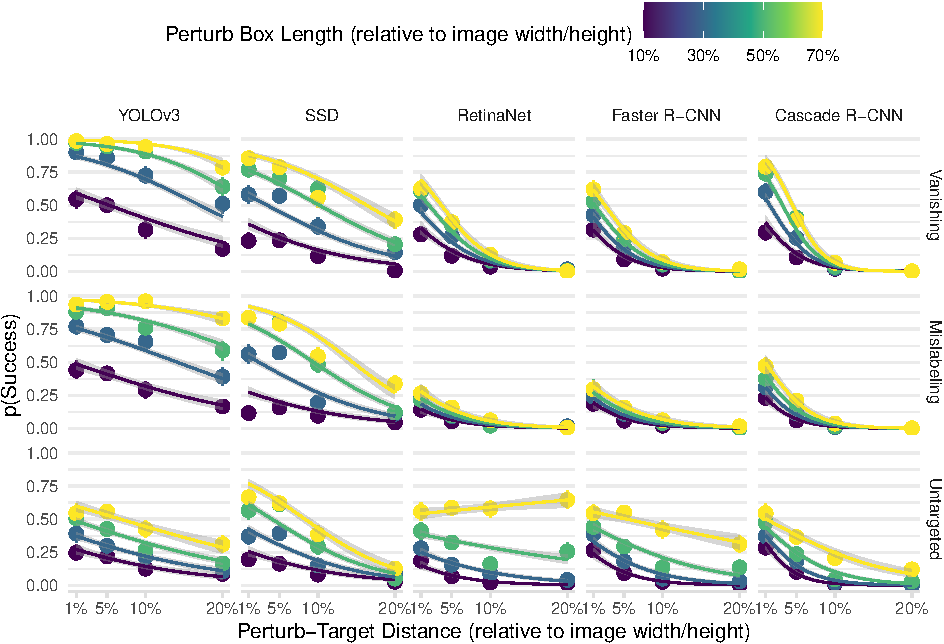
\includegraphics[width=1\linewidth]{rmd_imgs/arbitrary_trend_graph-1} 

}

\caption{\textbf{Perturbing an arbitrary region obfuscates intent with increased success for all models and attacks:}  We implement intent obfuscating attack by perturbing an arbitrary non-overlapping square region to disrupt a randomly selected target object at various lengths and distances. The binned summaries and regression trendlines graph success proportion against perturb-target distance and perturb box length, both relative to image width or height, in the deliberate attack experiment. Errors are 95\% confidence intervals and every point aggregates success over 200 images. The deliberate attack multiplies success as compared to the randomized attack (Figure \ref{fig:success_trend_graph}), especially at close perturb-target distance and large perturb box length, both relative to image width or height. Full details are given in Section \ref{sec:del_arb}.}\label{fig:arbitrary_trend_graph}
\end{figure}

\begingroup\fontsize{9}{11}\selectfont

\begin{longtable}[t]{llllrrrrrr}
\caption{\label{tab:rand_arb_compare_table}We combined the data in the randomized and deliberate attack experiments to run a logistic model regressing success against object (versus non-object), with perturb-target distance and perturb box size as covariates, both relative to image width or height. The ``object'' term codes object as 1 and non-object as 0. Perturbing an object (in the randomized attack) rather than a non-object (in the deliberate attack) significantly decreases success rates for all model and attack combinations, after controlling for perturb sizes and perturb-target distances. Table headers are explained in Appendix \ref{app:tab_hdr}.}\\
\toprule
\multicolumn{2}{c}{Group} & \multicolumn{8}{c}{Regression} \\
\cmidrule(l{3pt}r{3pt}){1-2} \cmidrule(l{3pt}r{3pt}){3-10}
 & Attack & term & sig & estimate & std.error & statistic & p.value & conf.low & conf.high\\
\midrule
\addlinespace[0.3em]
\multicolumn{10}{l}{\textbf{YOLOv3}}\\
\hspace{1em} & Vanishing & object & * & -1.058 & 0.069 & -15.371 & 0.000 & -1.193 & -0.924\\
\cmidrule{3-10}\nopagebreak
\hspace{1em} &  & distance & * & -8.585 & 0.514 & -16.712 & 0.000 & -9.607 & -7.594\\
\cmidrule{3-10}\nopagebreak
\hspace{1em} &  & size & * & 16.315 & 0.923 & 17.666 & 0.000 & 14.548 & 18.169\\
\cmidrule{3-10}\nopagebreak
\hspace{1em} &  & distance * size & * & -42.980 & 5.209 & -8.250 & 0.000 & -53.352 & -32.923\\
\cmidrule{2-10}\nopagebreak
\hspace{1em} & Mislabeling & object & * & -0.987 & 0.065 & -15.167 & 0.000 & -1.115 & -0.860\\
\cmidrule{3-10}\nopagebreak
\hspace{1em} &  & distance & * & -8.145 & 0.483 & -16.851 & 0.000 & -9.107 & -7.213\\
\cmidrule{3-10}\nopagebreak
\hspace{1em} &  & size & * & 9.168 & 0.560 & 16.364 & 0.000 & 8.093 & 10.290\\
\cmidrule{3-10}\nopagebreak
\hspace{1em} &  & distance * size & * & -9.986 & 3.571 & -2.796 & 0.005 & -17.040 & -3.037\\
\cmidrule{2-10}\nopagebreak
\hspace{1em} & Untargeted & object & * & -1.004 & 0.080 & -12.556 & 0.000 & -1.162 & -0.848\\
\cmidrule{3-10}\nopagebreak
\hspace{1em} &  & distance & * & -11.055 & 0.767 & -14.411 & 0.000 & -12.588 & -9.581\\
\cmidrule{3-10}\nopagebreak
\hspace{1em} &  & size & * & 2.759 & 0.294 & 9.375 & 0.000 & 2.185 & 3.339\\
\cmidrule{3-10}\nopagebreak
\hspace{1em} &  & distance * size & * & 11.988 & 2.700 & 4.439 & 0.000 & 6.717 & 17.305\\
\cmidrule{1-10}\pagebreak[0]
\addlinespace[0.3em]
\multicolumn{10}{l}{\textbf{SSD}}\\
\hspace{1em} & Vanishing & object & * & -0.571 & 0.064 & -8.877 & 0.000 & -0.697 & -0.445\\
\cmidrule{3-10}\nopagebreak
\hspace{1em} &  & distance & * & -13.706 & 0.651 & -21.064 & 0.000 & -15.003 & -12.452\\
\cmidrule{3-10}\nopagebreak
\hspace{1em} &  & size & * & 5.147 & 0.375 & 13.729 & 0.000 & 4.423 & 5.893\\
\cmidrule{3-10}\nopagebreak
\hspace{1em} &  & distance * size &  & 4.541 & 2.991 & 1.518 & 0.129 & -1.327 & 10.401\\
\cmidrule{2-10}\nopagebreak
\hspace{1em} & Mislabeling & object & * & -1.064 & 0.067 & -15.825 & 0.000 & -1.196 & -0.932\\
\cmidrule{3-10}\nopagebreak
\hspace{1em} &  & distance & * & -14.437 & 0.728 & -19.818 & 0.000 & -15.889 & -13.032\\
\cmidrule{3-10}\nopagebreak
\hspace{1em} &  & size & * & 5.207 & 0.378 & 13.786 & 0.000 & 4.477 & 5.958\\
\cmidrule{3-10}\nopagebreak
\hspace{1em} &  & distance * size &  & 2.193 & 3.132 & 0.700 & 0.484 & -3.950 & 8.334\\
\cmidrule{2-10}\nopagebreak
\hspace{1em} & Untargeted & object & * & -0.905 & 0.069 & -13.072 & 0.000 & -1.041 & -0.769\\
\cmidrule{3-10}\nopagebreak
\hspace{1em} &  & distance & * & -14.758 & 0.791 & -18.656 & 0.000 & -16.336 & -13.235\\
\cmidrule{3-10}\nopagebreak
\hspace{1em} &  & size & * & 2.899 & 0.299 & 9.704 & 0.000 & 2.318 & 3.489\\
\cmidrule{3-10}\nopagebreak
\hspace{1em} &  & distance * size & * & 14.317 & 2.905 & 4.929 & 0.000 & 8.639 & 20.028\\
\cmidrule{1-10}\pagebreak[0]
\addlinespace[0.3em]
\multicolumn{10}{l}{\textbf{RetinaNet}}\\
\hspace{1em} & Vanishing & object & * & -0.722 & 0.091 & -7.952 & 0.000 & -0.901 & -0.545\\
\cmidrule{3-10}\nopagebreak
\hspace{1em} &  & distance & * & -26.079 & 1.694 & -15.391 & 0.000 & -29.487 & -22.845\\
\cmidrule{3-10}\nopagebreak
\hspace{1em} &  & size & * & 3.679 & 0.368 & 9.987 & 0.000 & 2.964 & 4.409\\
\cmidrule{3-10}\nopagebreak
\hspace{1em} &  & distance * size &  & -11.595 & 6.212 & -1.866 & 0.062 & -23.913 & 0.450\\
\cmidrule{2-10}\nopagebreak
\hspace{1em} & Mislabeling & object & * & -0.658 & 0.128 & -5.152 & 0.000 & -0.912 & -0.411\\
\cmidrule{3-10}\nopagebreak
\hspace{1em} &  & distance & * & -25.807 & 2.486 & -10.383 & 0.000 & -30.879 & -21.136\\
\cmidrule{3-10}\nopagebreak
\hspace{1em} &  & size & * & 2.177 & 0.424 & 5.132 & 0.000 & 1.347 & 3.010\\
\cmidrule{3-10}\nopagebreak
\hspace{1em} &  & distance * size &  & -9.894 & 9.044 & -1.094 & 0.274 & -27.848 & 7.624\\
\cmidrule{2-10}\nopagebreak
\hspace{1em} & Untargeted & object & * & -0.700 & 0.082 & -8.497 & 0.000 & -0.862 & -0.539\\
\cmidrule{3-10}\nopagebreak
\hspace{1em} &  & distance & * & -11.600 & 0.898 & -12.914 & 0.000 & -13.402 & -9.881\\
\cmidrule{3-10}\nopagebreak
\hspace{1em} &  & size & * & 3.774 & 0.298 & 12.674 & 0.000 & 3.193 & 4.361\\
\cmidrule{3-10}\nopagebreak
\hspace{1em} &  & distance * size & * & 24.806 & 2.869 & 8.645 & 0.000 & 19.250 & 30.502\\
\cmidrule{1-10}\pagebreak[0]
\addlinespace[0.3em]
\multicolumn{10}{l}{\textbf{Faster R-CNN}}\\
\hspace{1em} & Vanishing & object & * & -1.151 & 0.116 & -9.929 & 0.000 & -1.382 & -0.927\\
\cmidrule{3-10}\nopagebreak
\hspace{1em} &  & distance & * & -23.384 & 1.894 & -12.347 & 0.000 & -27.219 & -19.793\\
\cmidrule{3-10}\nopagebreak
\hspace{1em} &  & size & * & 3.854 & 0.399 & 9.653 & 0.000 & 3.079 & 4.644\\
\cmidrule{3-10}\nopagebreak
\hspace{1em} &  & distance * size & * & -30.041 & 7.548 & -3.980 & 0.000 & -45.026 & -15.421\\
\cmidrule{2-10}\nopagebreak
\hspace{1em} & Mislabeling & object & * & -1.120 & 0.144 & -7.777 & 0.000 & -1.409 & -0.843\\
\cmidrule{3-10}\nopagebreak
\hspace{1em} &  & distance & * & -20.020 & 2.071 & -9.666 & 0.000 & -24.249 & -16.130\\
\cmidrule{3-10}\nopagebreak
\hspace{1em} &  & size & * & 2.173 & 0.418 & 5.203 & 0.000 & 1.355 & 2.992\\
\cmidrule{3-10}\nopagebreak
\hspace{1em} &  & distance * size & * & -20.523 & 8.353 & -2.457 & 0.014 & -37.166 & -4.402\\
\cmidrule{2-10}\nopagebreak
\hspace{1em} & Untargeted & object & * & -1.063 & 0.090 & -11.807 & 0.000 & -1.241 & -0.888\\
\cmidrule{3-10}\nopagebreak
\hspace{1em} &  & distance & * & -14.346 & 0.989 & -14.512 & 0.000 & -16.324 & -12.449\\
\cmidrule{3-10}\nopagebreak
\hspace{1em} &  & size & * & 2.995 & 0.307 & 9.759 & 0.000 & 2.396 & 3.600\\
\cmidrule{3-10}\nopagebreak
\hspace{1em} &  & distance * size & * & 31.094 & 3.055 & 10.177 & 0.000 & 25.172 & 37.154\\
\cmidrule{1-10}\pagebreak[0]
\addlinespace[0.3em]
\multicolumn{10}{l}{\textbf{Cascade R-CNN}}\\
\hspace{1em} & Vanishing & object & * & -1.264 & 0.104 & -12.174 & 0.000 & -1.469 & -1.062\\
\cmidrule{3-10}\nopagebreak
\hspace{1em} &  & distance & * & -30.978 & 2.091 & -14.812 & 0.000 & -35.190 & -26.993\\
\cmidrule{3-10}\nopagebreak
\hspace{1em} &  & size & * & 5.672 & 0.447 & 12.682 & 0.000 & 4.810 & 6.565\\
\cmidrule{3-10}\nopagebreak
\hspace{1em} &  & distance * size & * & -54.045 & 8.997 & -6.007 & 0.000 & -72.015 & -36.715\\
\cmidrule{2-10}\nopagebreak
\hspace{1em} & Mislabeling & object & * & -1.181 & 0.126 & -9.392 & 0.000 & -1.431 & -0.938\\
\cmidrule{3-10}\nopagebreak
\hspace{1em} &  & distance & * & -30.703 & 2.729 & -11.252 & 0.000 & -36.258 & -25.562\\
\cmidrule{3-10}\nopagebreak
\hspace{1em} &  & size & * & 3.894 & 0.400 & 9.736 & 0.000 & 3.116 & 4.684\\
\cmidrule{3-10}\nopagebreak
\hspace{1em} &  & distance * size & * & -28.704 & 9.725 & -2.952 & 0.003 & -47.925 & -9.780\\
\cmidrule{2-10}\nopagebreak
\hspace{1em} & Untargeted & object & * & -0.853 & 0.098 & -8.720 & 0.000 & -1.047 & -0.663\\
\cmidrule{3-10}\nopagebreak
\hspace{1em} &  & distance & * & -24.912 & 1.590 & -15.672 & 0.000 & -28.113 & -21.881\\
\cmidrule{3-10}\nopagebreak
\hspace{1em} &  & size & * & 1.999 & 0.306 & 6.526 & 0.000 & 1.400 & 2.601\\
\cmidrule{3-10}\nopagebreak
\hspace{1em} &  & distance * size & * & 35.071 & 4.099 & 8.556 & 0.000 & 27.118 & 43.194\\
\bottomrule
\end{longtable}
\endgroup{}

\end{document}
